\documentclass[
	fontsize=12pt,
	paper=a4,
	twoside=false,
	numbers=noenddot,
	plainheadsepline,
	toc=listof,
	toc=bibliography
]{scrartcl}

\usepackage[english]{babel} 

\usepackage[round]{natbib}

\usepackage{amssymb,amsmath}

\usepackage{placeins}
\usepackage{float}

\usepackage{graphicx}
\restylefloat{figure}
\usepackage{subfigure} 

\usepackage{array}

\usepackage{hyperref}

\setlength{\parindent}{0pt}

\title{Testing Reweighted Random Walk Method (RRWM) for Graph Matching }


\begin{document}

\maketitle

We consider two graphs $G_1=(V, D, E)$ and $G_2=(V, D, E)$, where $V = \{v_i\}_{i=1}^{n_1(n_2)}$ is the set of nodes, $D= \{d_i\}_{i=1}^{n_1(n_2)}$ is the set of node attributes and $E = \{e_{j}\}_{j=1}^{m_1(m_2)}$ is the set of graph edges.

We want to test the behaviour of the $RRWM$ in case of matching two graphs with a common sub-graph.
The results of tests are represented below.
In the first case, graphs $G_1$ and $G_2$ are almost similar (except for one additional node and missing edge in $G_2$). In the second and third tests, one graph is a sub-graph of the other. In the fourth case both graphs have a common sub-graph.

We can see, that RRWM had achieved good results in all case. Notable, that the algorithm was able to detect common structure of the graphs in all tests.
\newpage
% ----------------------------------------------------------------------------------
\subsection*{ Case $1$: $V(G_1)\cap V(G2) = V(G_1)$, $n_1=17$, $n_2=18$}
% ----------------------------------------------------------------------------------

\begin{figure} [htb] \centering
	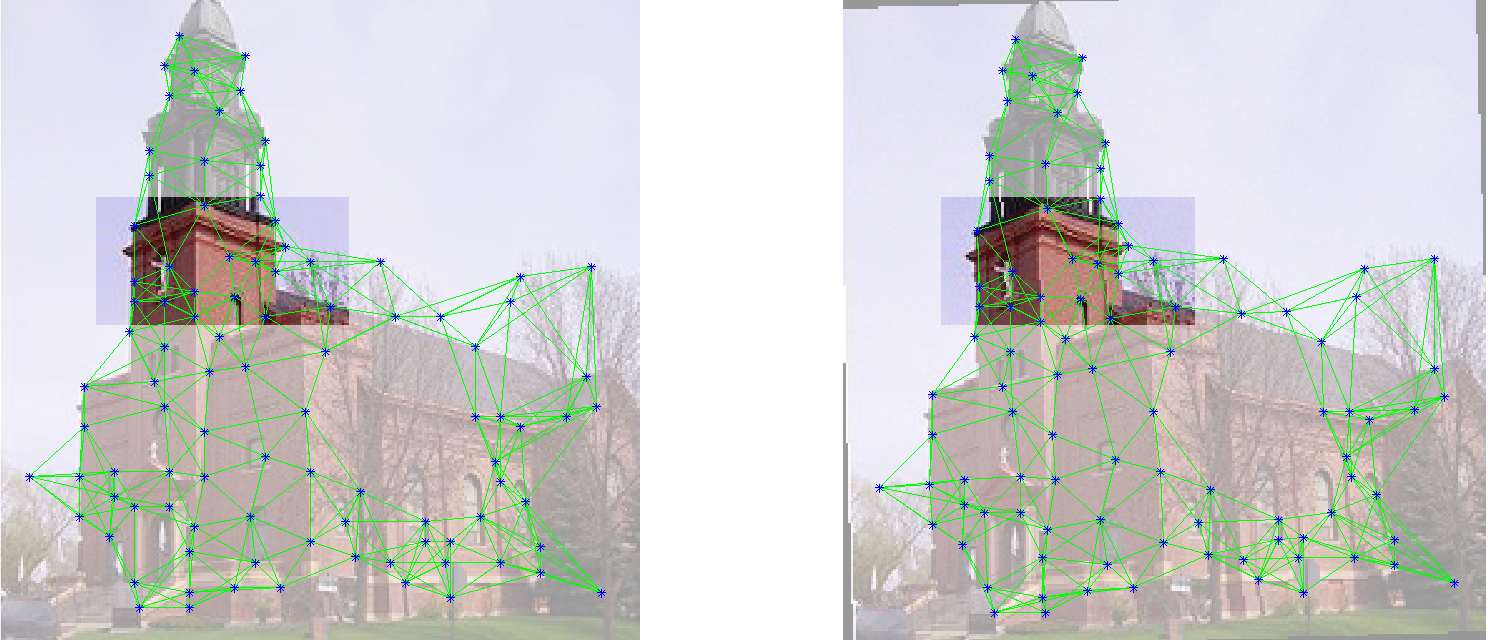
\includegraphics[scale = 0.3]{test1/subregions.png}
\end{figure}
\begin{figure} [hb] \centering
	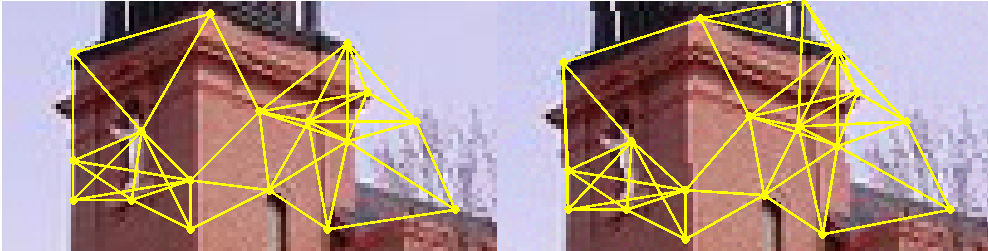
\includegraphics[scale = 0.4]{test1/subgraphs.png}
	\caption{Graphs $G_1$ and $G_2$}
\end{figure}
\begin{figure} [hb] \centering
	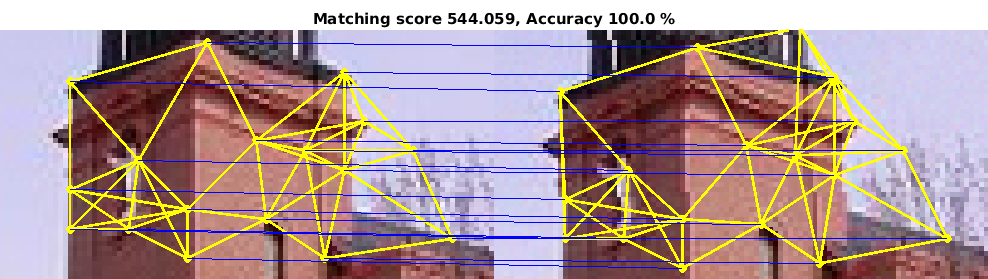
\includegraphics[scale = 0.4]{test1/matching_result.png}
	\caption{ Matching result}
\end{figure}

\FloatBarrier

\newpage
% ----------------------------------------------------------------------------------
\subsection*{ Case $2$: $V(G_1)\cap V(G2) = V(G_1)$, $n_1=17$, $n_2=21$}
% ----------------------------------------------------------------------------------
\begin{figure} [htb] \centering
	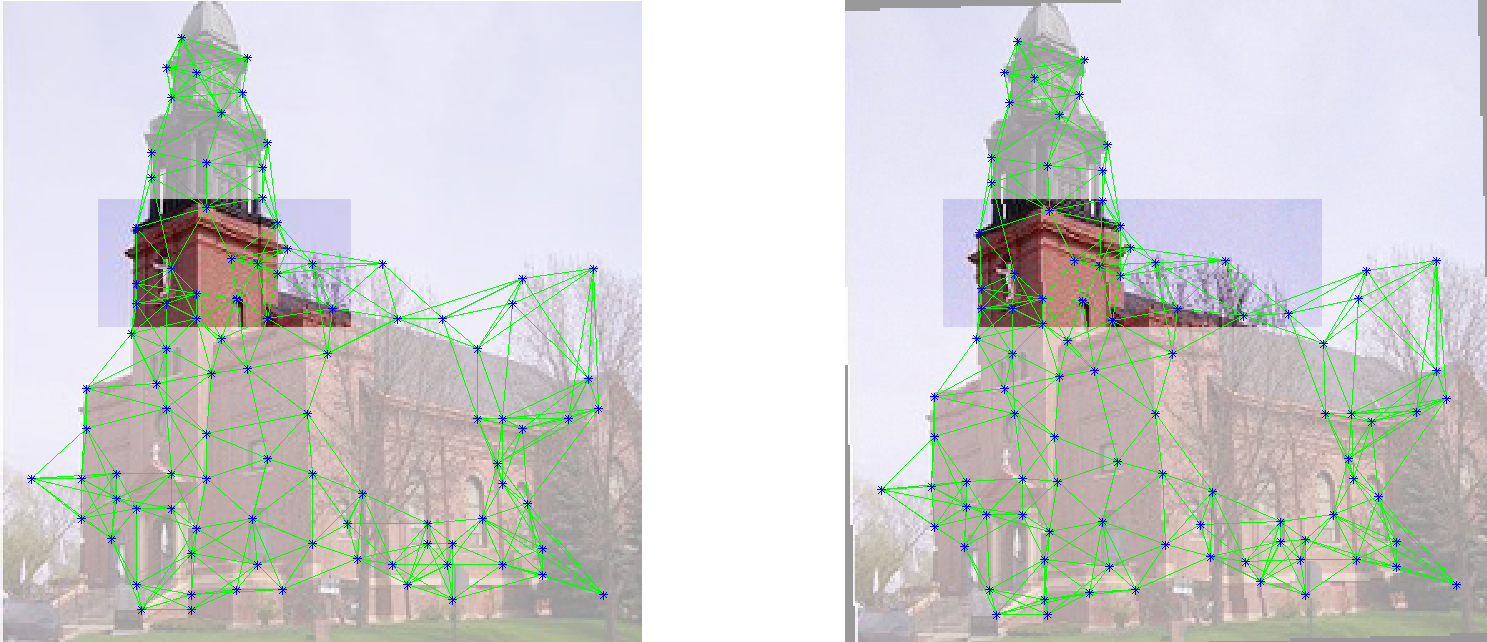
\includegraphics[scale = 0.35]{test2/subregions.png}
\end{figure}
\begin{figure} [hb] \centering
	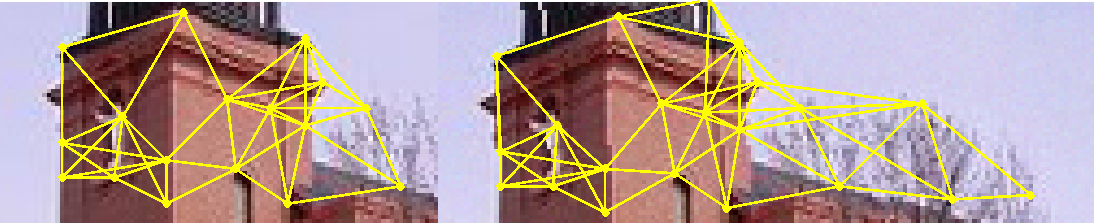
\includegraphics[scale = 0.4]{test2/subgraphs.png}
	\caption{Graphs $G_1$ and $G_2$}
\end{figure}
\begin{figure} [hb] \centering
	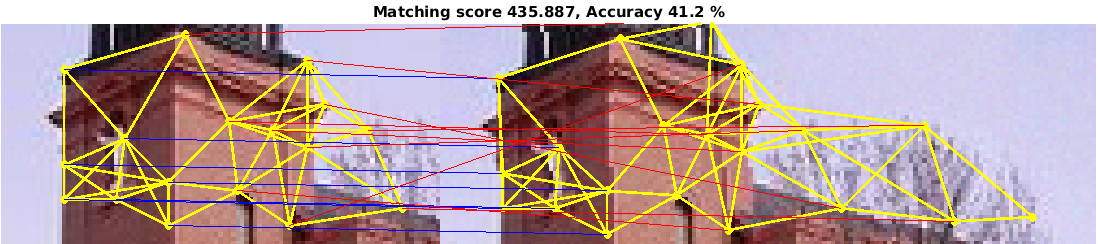
\includegraphics[scale = 0.4]{test2/matching_result.png}
	\caption{ Matching result}
\end{figure}

\FloatBarrier

\newpage
% ----------------------------------------------------------------------------------
\subsection*{ Case $3$: $V(G_1)\cap V(G2) = V(G_2)\setminus\{v\}$, $n_1=23$, $n_2=18$}
% ----------------------------------------------------------------------------------
\begin{figure} [htb] \centering
	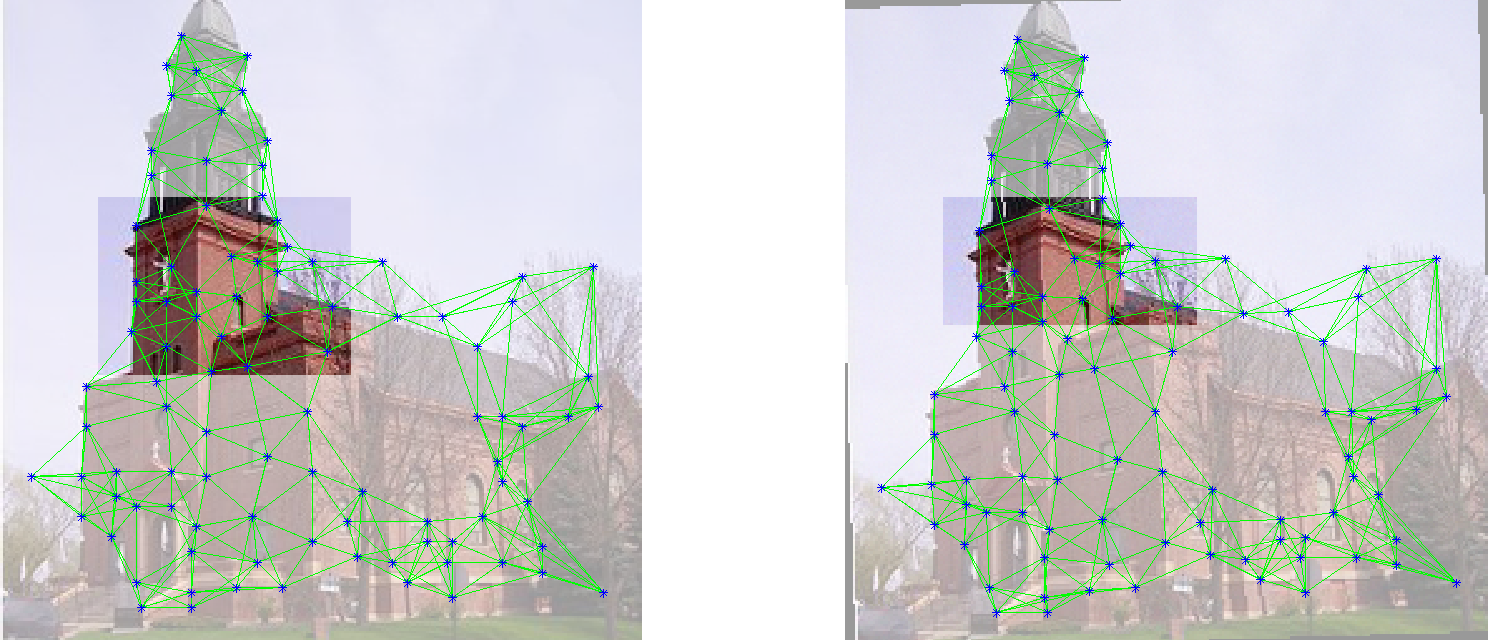
\includegraphics[scale = 0.35]{test3/subregions.png}
\end{figure}
\begin{figure} [hb] \centering
	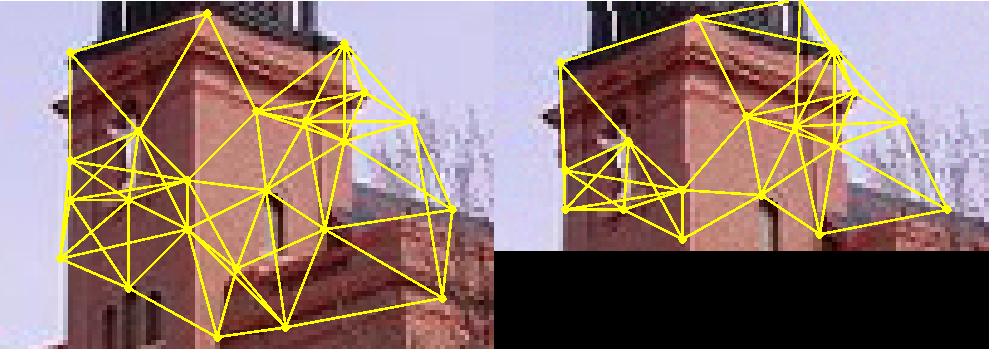
\includegraphics[scale = 0.4]{test3/subgraphs.png}
	\caption{Graphs $G_1$ and $G_2$}
\end{figure}
\begin{figure} [htb] \centering
	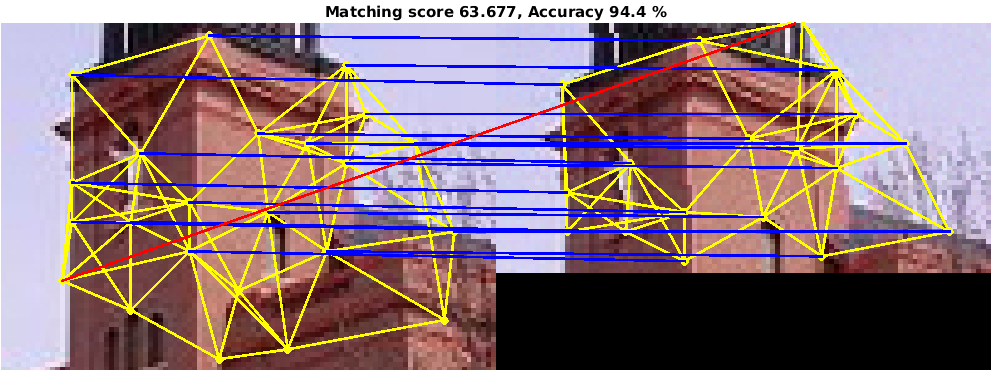
\includegraphics[scale = 0.4]{test3/matching_result.png}
	\caption{ Matching result}
\end{figure}

\FloatBarrier

\newpage
% ----------------------------------------------------------------------------------
\subsection*{ Case $4$: $V(G_1)\cap V(G2) = V(H)$, $H\subset G_1$, $H\subset G_2$}
% ----------------------------------------------------------------------------------
\begin{figure} [htb] \centering
	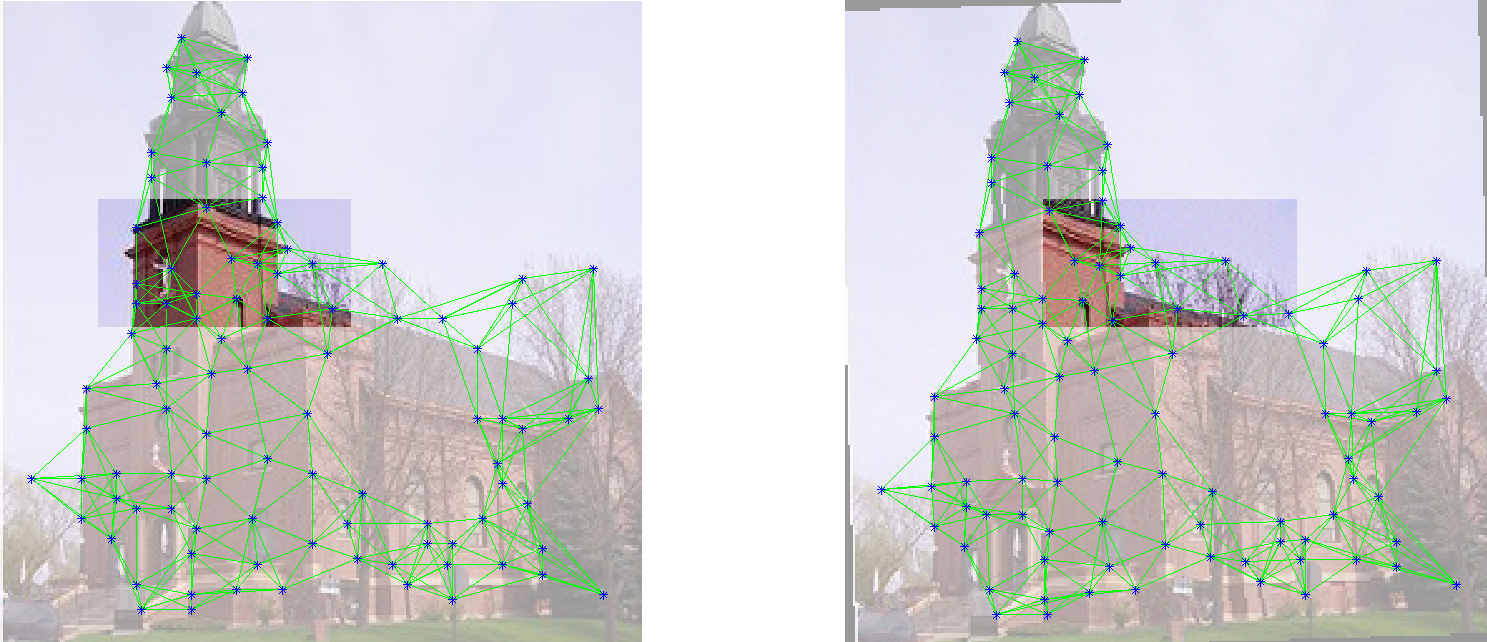
\includegraphics[scale = 0.35]{test4/subregions.png}
\end{figure}
\begin{figure} [hb] \centering
	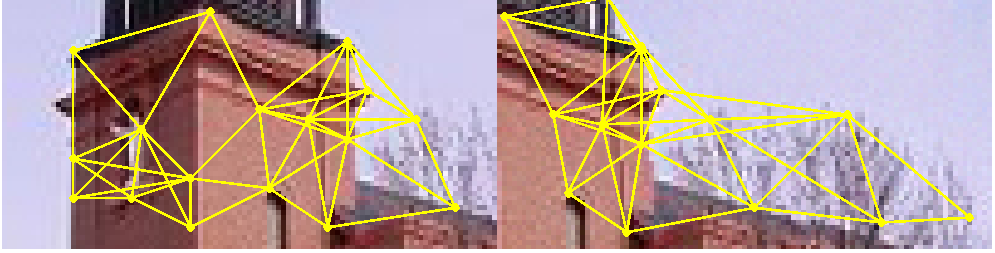
\includegraphics[scale = 0.4]{test4/subgraphs.png}
	\caption{Graphs $G_1$ and $G_2$}
\end{figure}
\begin{figure} [htb] \centering
	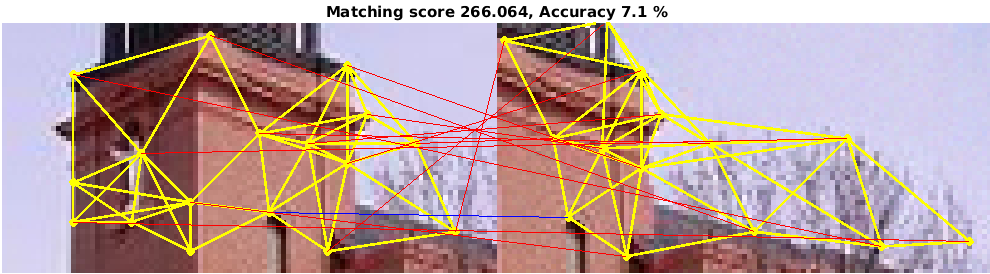
\includegraphics[scale = 0.4]{test4/matching_result.png}
	\caption{ Matching result}
\end{figure}

\FloatBarrier

\begin{figure} [htb] \centering
	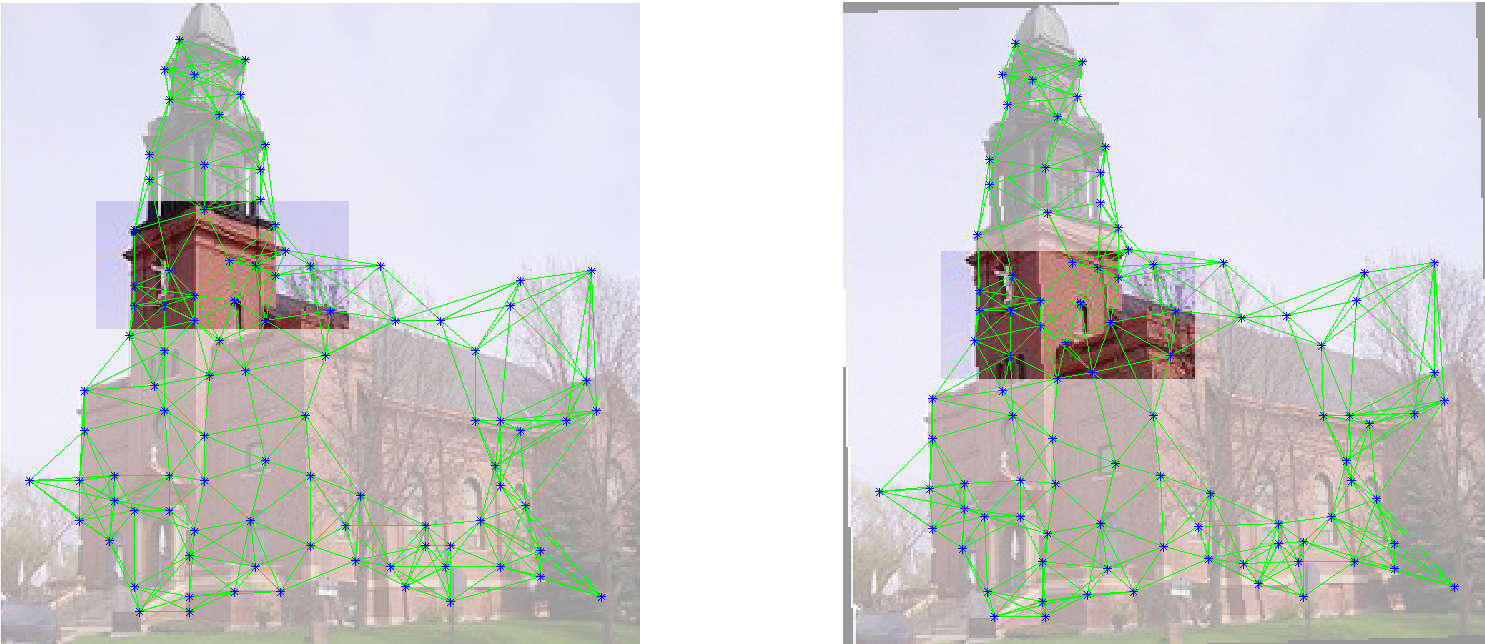
\includegraphics[scale = 0.35]{test5/subregions.png}
\end{figure}
\begin{figure} [hb] \centering
	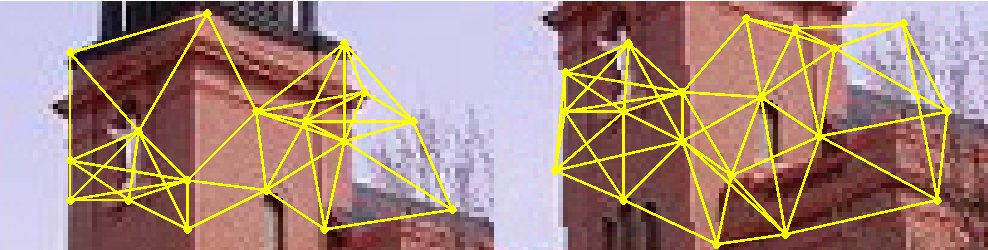
\includegraphics[scale = 0.4]{test5/subgraphs.png}
	\caption{Graphs $G_1$ and $G_2$}
\end{figure}
\begin{figure} [htb] \centering
	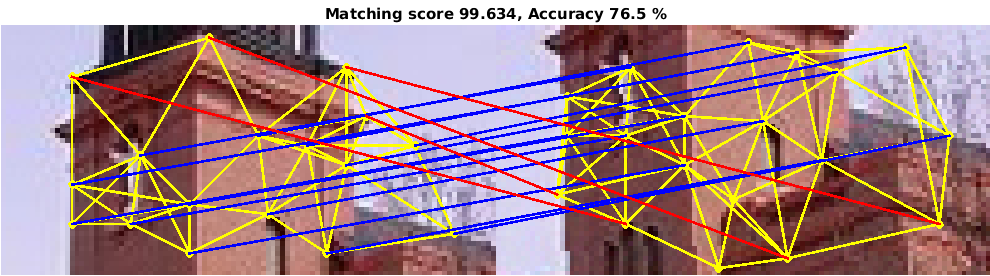
\includegraphics[scale = 0.4]{test5/matching_result.png}
	\caption{ Matching result}
\end{figure}

\FloatBarrier

\begin{figure} [htb] \centering
	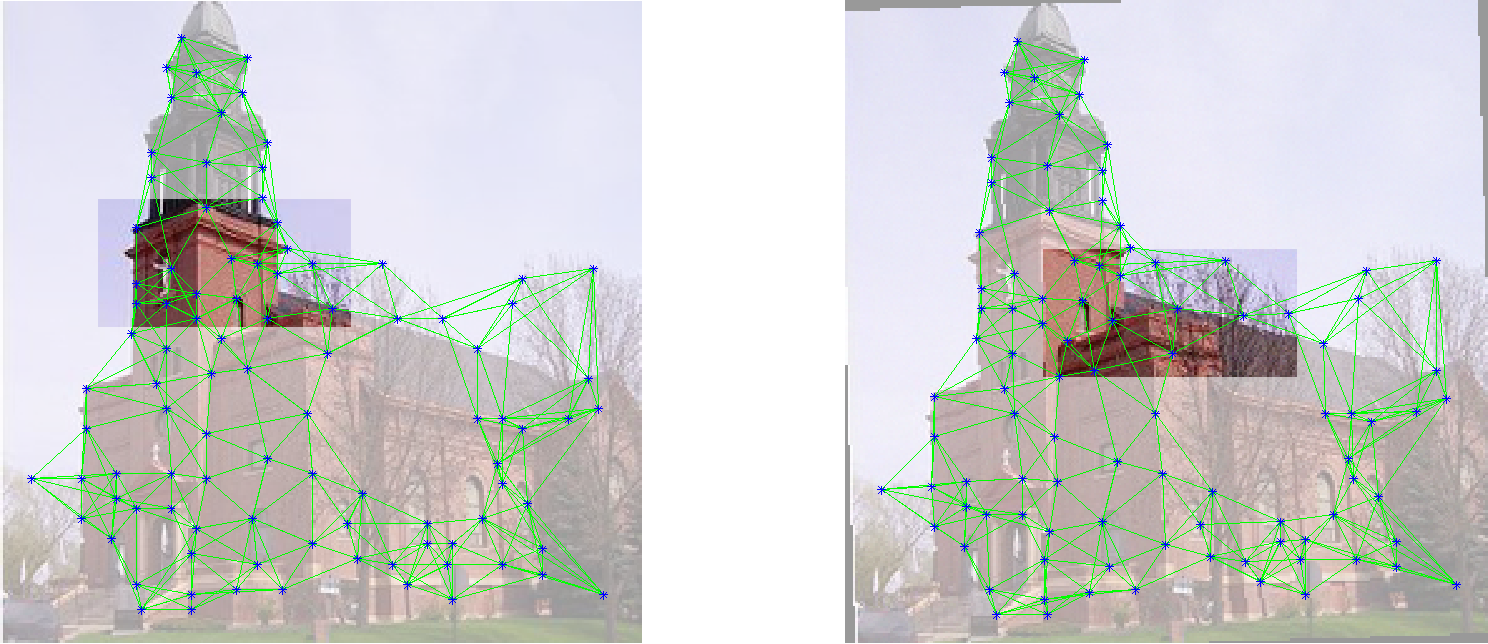
\includegraphics[scale = 0.35]{test6/subregions.png}
\end{figure}
\begin{figure} [hb] \centering
	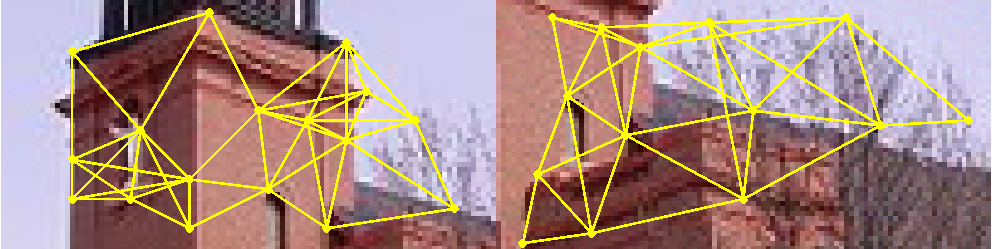
\includegraphics[scale = 0.4]{test6/subgraphs.png}
	\caption{Graphs $G_1$ and $G_2$}
\end{figure}
\begin{figure} [htb] \centering
	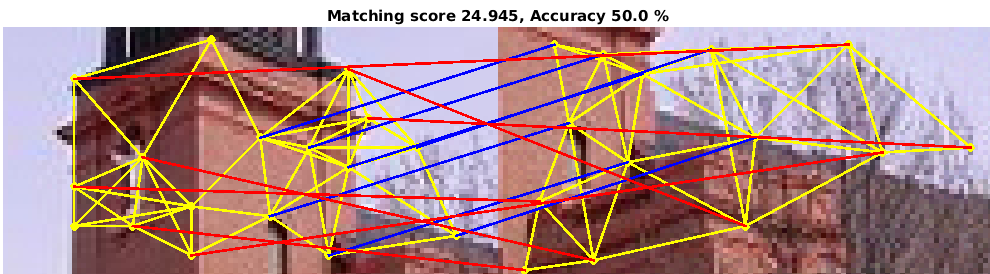
\includegraphics[scale = 0.4]{test6/matching_result.png}
	\caption{ Matching result}
\end{figure}

\FloatBarrier

\end{document}